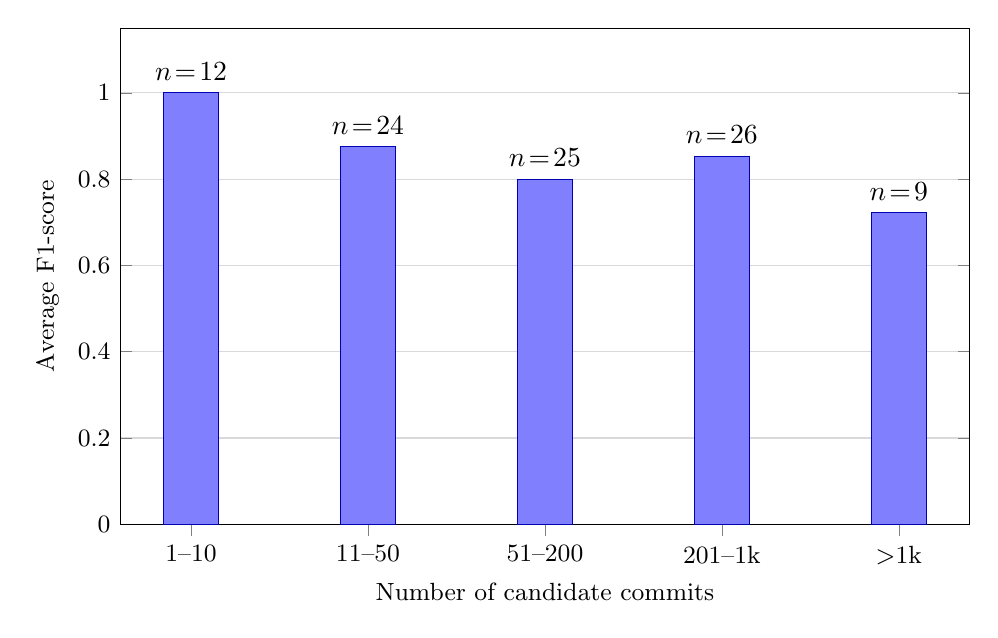
\begin{tikzpicture}
\begin{axis}[
    width=1.02\columnwidth,
    height=0.65\columnwidth,
    ybar,
    bar width=20pt,
    xlabel={Number of candidate commits},
    ylabel={Average F1-score},
    ymin=0, ymax=1.15,
    ytick={0, 0.2, 0.4, 0.6, 0.8, 1.0},
    symbolic x coords={1--10,11--50,51--200,201--1k,{$>$1k}},
    xtick=data,
    x tick label style={font=\small},
    tick label style={font=\small},
    label style={font=\small},
    grid=major,
    grid style={gray!30},
    ymajorgrids=true,
    xmajorgrids=false,
    nodes near coords={\scriptsize $n\!=\!{}$},
    every node near coord/.append style={anchor=south, yshift=1pt},
    xtick pos=left,
]
\addplot[
    fill=blue!50,
    draw=blue!70!black,
    point meta=explicit symbolic,
    nodes near coords={\pgfplotspointmeta},
] coordinates {
    (1--10, 1.000) [$n\!=\!12$]
    (11--50, 0.875) [$n\!=\!24$]
    (51--200, 0.800) [$n\!=\!25$]
    (201--1k, 0.853) [$n\!=\!26$]
    ({$>$1k}, 0.722) [$n\!=\!9$]
};
\end{axis}
\end{tikzpicture}
